\section{第六章}

\subsection{题目1}

求$y'=1+y^2,y(0)=0$的数值解(分别用欧拉显格式、梯形预估修正格式、4阶龙格库塔格式,并与解析解比较这三种格式的收敛性)

\paragraph{欧拉显式格式}:
\subparagraph{公式推导}
根据泰勒展开, 有

$$y\left(t_{j+1}\right) + hf\left(t_j,y\left(t_j\right)\right) + \frac{h^2}{2}y^{''}\left(\xi_j\right)$$

忽略余项, 可以得到欧拉显式格式:

$$\left\{
\begin{aligned}
w_0 &= \alpha \\
w_{j+1} &= w_j + hf\left(t_j,w_j\right)
\end{aligned}
\right.$$

\subparagraph{误差分析}

假设 $f$在$D = \left\{\left(t,y\right) \big{|} a \leq t \leq b,-\infty < y < \infty \right\}$连续,满足Lipschitz条件(Lipschitz常数为$L$),且满足$\left|y^{''}\left(t\right) \right| \leq M,\forall t\in \left[a,b\right]$. 则$\left|y\left(t_j\right) - w_j \right| \leq \frac{hM}{2L}\left[ e^{L\left(t_j-a\right)}-1\right]$.在某些情况下, $M,L$较难确定. 但可以发现, 随着向后递推, 欧拉显式格式的误差逐渐增大。

\subparagraph{欧拉法误差分析}

对于$$\left|y\left(x_j\right) - w_j \right| \leq \frac{hM}{2L}\left[ e^{L\left(x_j-a\right)}-1\right]$$, 需要确定$M,L$的值.

由于$$M = \max \left|y^{''}\left(x\right) \right|,x\in \left[a,b\right]$$,

而$$y\left(x\right) = \sqrt{2x+1}$$,$$y^{''}\left(x\right) = \frac{-1}{\left(2x+1\right)^{3/2}}$$

有$$M = \max \left|y^{''}\left(x\right) \right| = \left|f^{''}\left(-1\right)\right| = 1$$

$$ \frac{\partial f}{\partial y} = 1+\frac{2x}{y^2} = 1+\frac{2x}{1+2x}$$, $$L = \max \left|\frac{\partial f}{\partial y} \right| = \left|\frac{\partial f}{\partial y} \big{|}_{x=1} \right| \approx 1.6667$$.

因此$$\left|y\left(1\right) - w_{n} \right| \leq \frac{hM}{2L}\left[ e^{L}-1\right] $$。

\paragraph{梯形预估修正格式}

利用数值积分方法将微分方程离散化时,若用梯形公式计算右端积分,即
$$\int_{x_{n}}^{x_{m 1}} f(x, y(x)) d x \approx \frac{h}{2}\left[f\left(x_{n}, y\left(x_{n}\right)\right)+f\left(x_{n+1}, y\left(x_{n+1}\right)\right)\right]$$
并用$y_n,y_{n+1}$代替$y(x_n),y(x_{n+1})$,则得计算公式
$$y_{n+1}=y_{n}+\frac{h}{2}\left[f\left(x_{n}, y_{n}\right)+f\left(x_{n+1}, y_{n+1}\right)\right]$$
这就是梯形预估修正格式。由于梯形公式仍是隐式格式,一般需用迭代法求解,迭代公式为

$$\left \{ \begin{array}{l}{y_{n+1}^{(0)}=y_{n}+h f\left(x_{n}, y_{n}\right)} \\ {y_{n+1}^{(k+1)}=y_{n}+\frac{h}{2}\left[f\left(x_{n}, y_{n}\right)+f\left(x_{n+1}, y_{n+1}^{(k)}\right)\right]} \\ {(k=0,1,2, \cdots)}\end{array}\right.$$

\paragraph{4阶龙格库塔格式}

对于方程$y'=f(x)$,存在a,其中$x_n<a<x_{n+1}$,有$\frac{y(x_{n+1})-y(x_n)}{h}=y'=f(x)$,为了提高y的精度,我们令
$$K_1=f(x_n,y_n)$$$$K_2=f(x_{n+\frac{1}{2}},y_n+\frac{h}{2}K_1)$$$$K_3=f(x_{n+\frac{1}{2}},y_n+\frac{h}{2}K_1)$$$$K_4=f(x_{n+1},y_n+hK_3)$$$$y_{n+1}=y_n+\frac{h}{6}(K_1+2K_2+2K_3+K_4)$$


\paragraph{解答}


使用欧拉显格式对于$y'=1+y^2,y(0)=0$求数值解得下拟合图:

\begin{figure}[H]
	\centering
	\caption{欧拉显格式}
	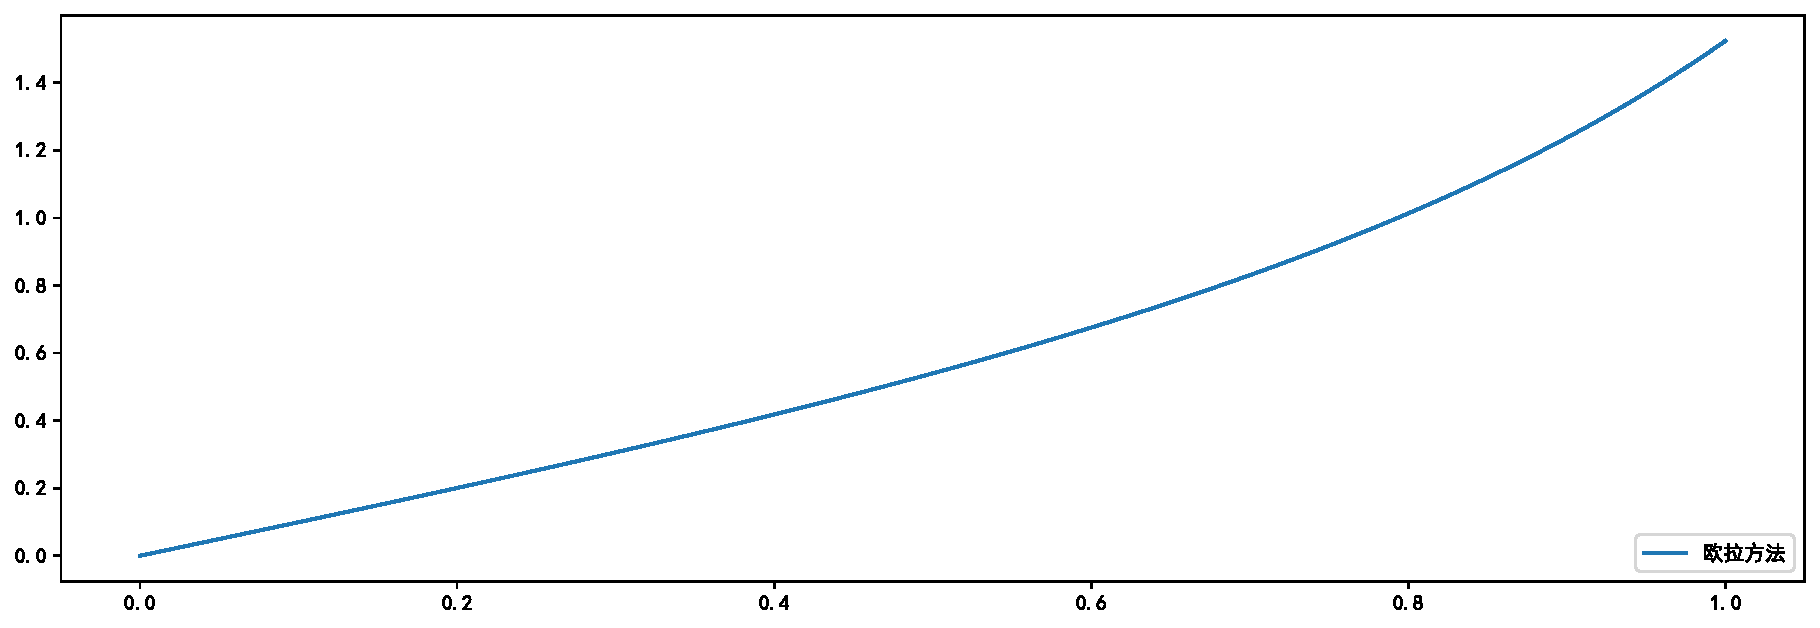
\includegraphics[width=\linewidth]{6-1.pdf}
\end{figure}

使用4阶龙格库塔格式对于$y'=1+y^2,y(0)=0$求数值解得下拟合图:

\begin{figure}[H]
	\centering
	\caption{4阶龙格库塔格式}
	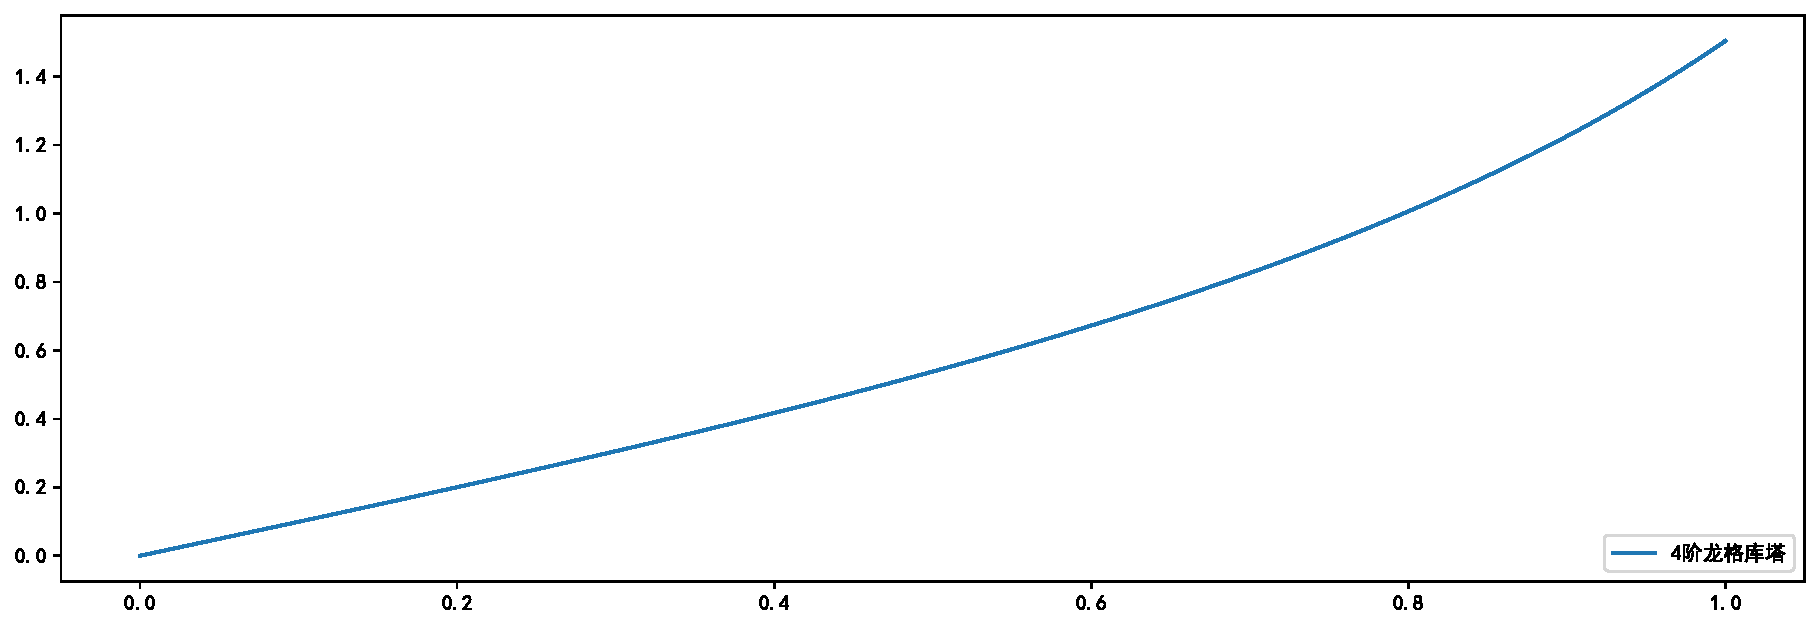
\includegraphics[width=\linewidth]{6-2.pdf}
\end{figure}

使用梯形预估修正格式对于$y'=1+y^2,y(0)=0$求数值解得下拟合图:

\begin{figure}[H]
	\centering
	\caption{梯形预估修正格式}
	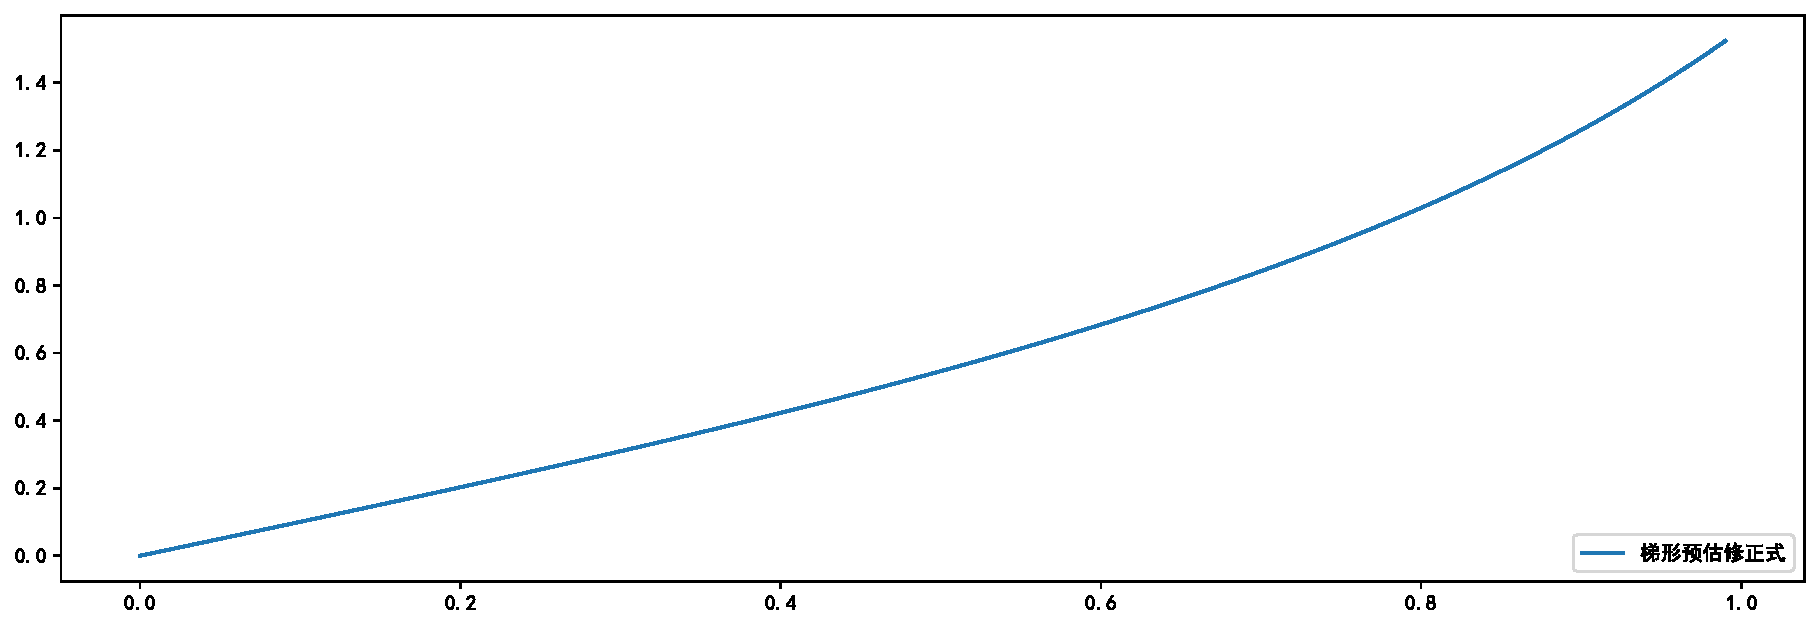
\includegraphics[width=\linewidth]{6-3.pdf}
\end{figure}






对方程求解得,y=tan(x).取h=0.01,分别利用欧拉显格式、梯形预估修正格式和4阶龙格库塔格式计算对应的解,绘制下图:


\begin{figure}[H]
	\centering
	\caption{3种方法与原函数的图像}
	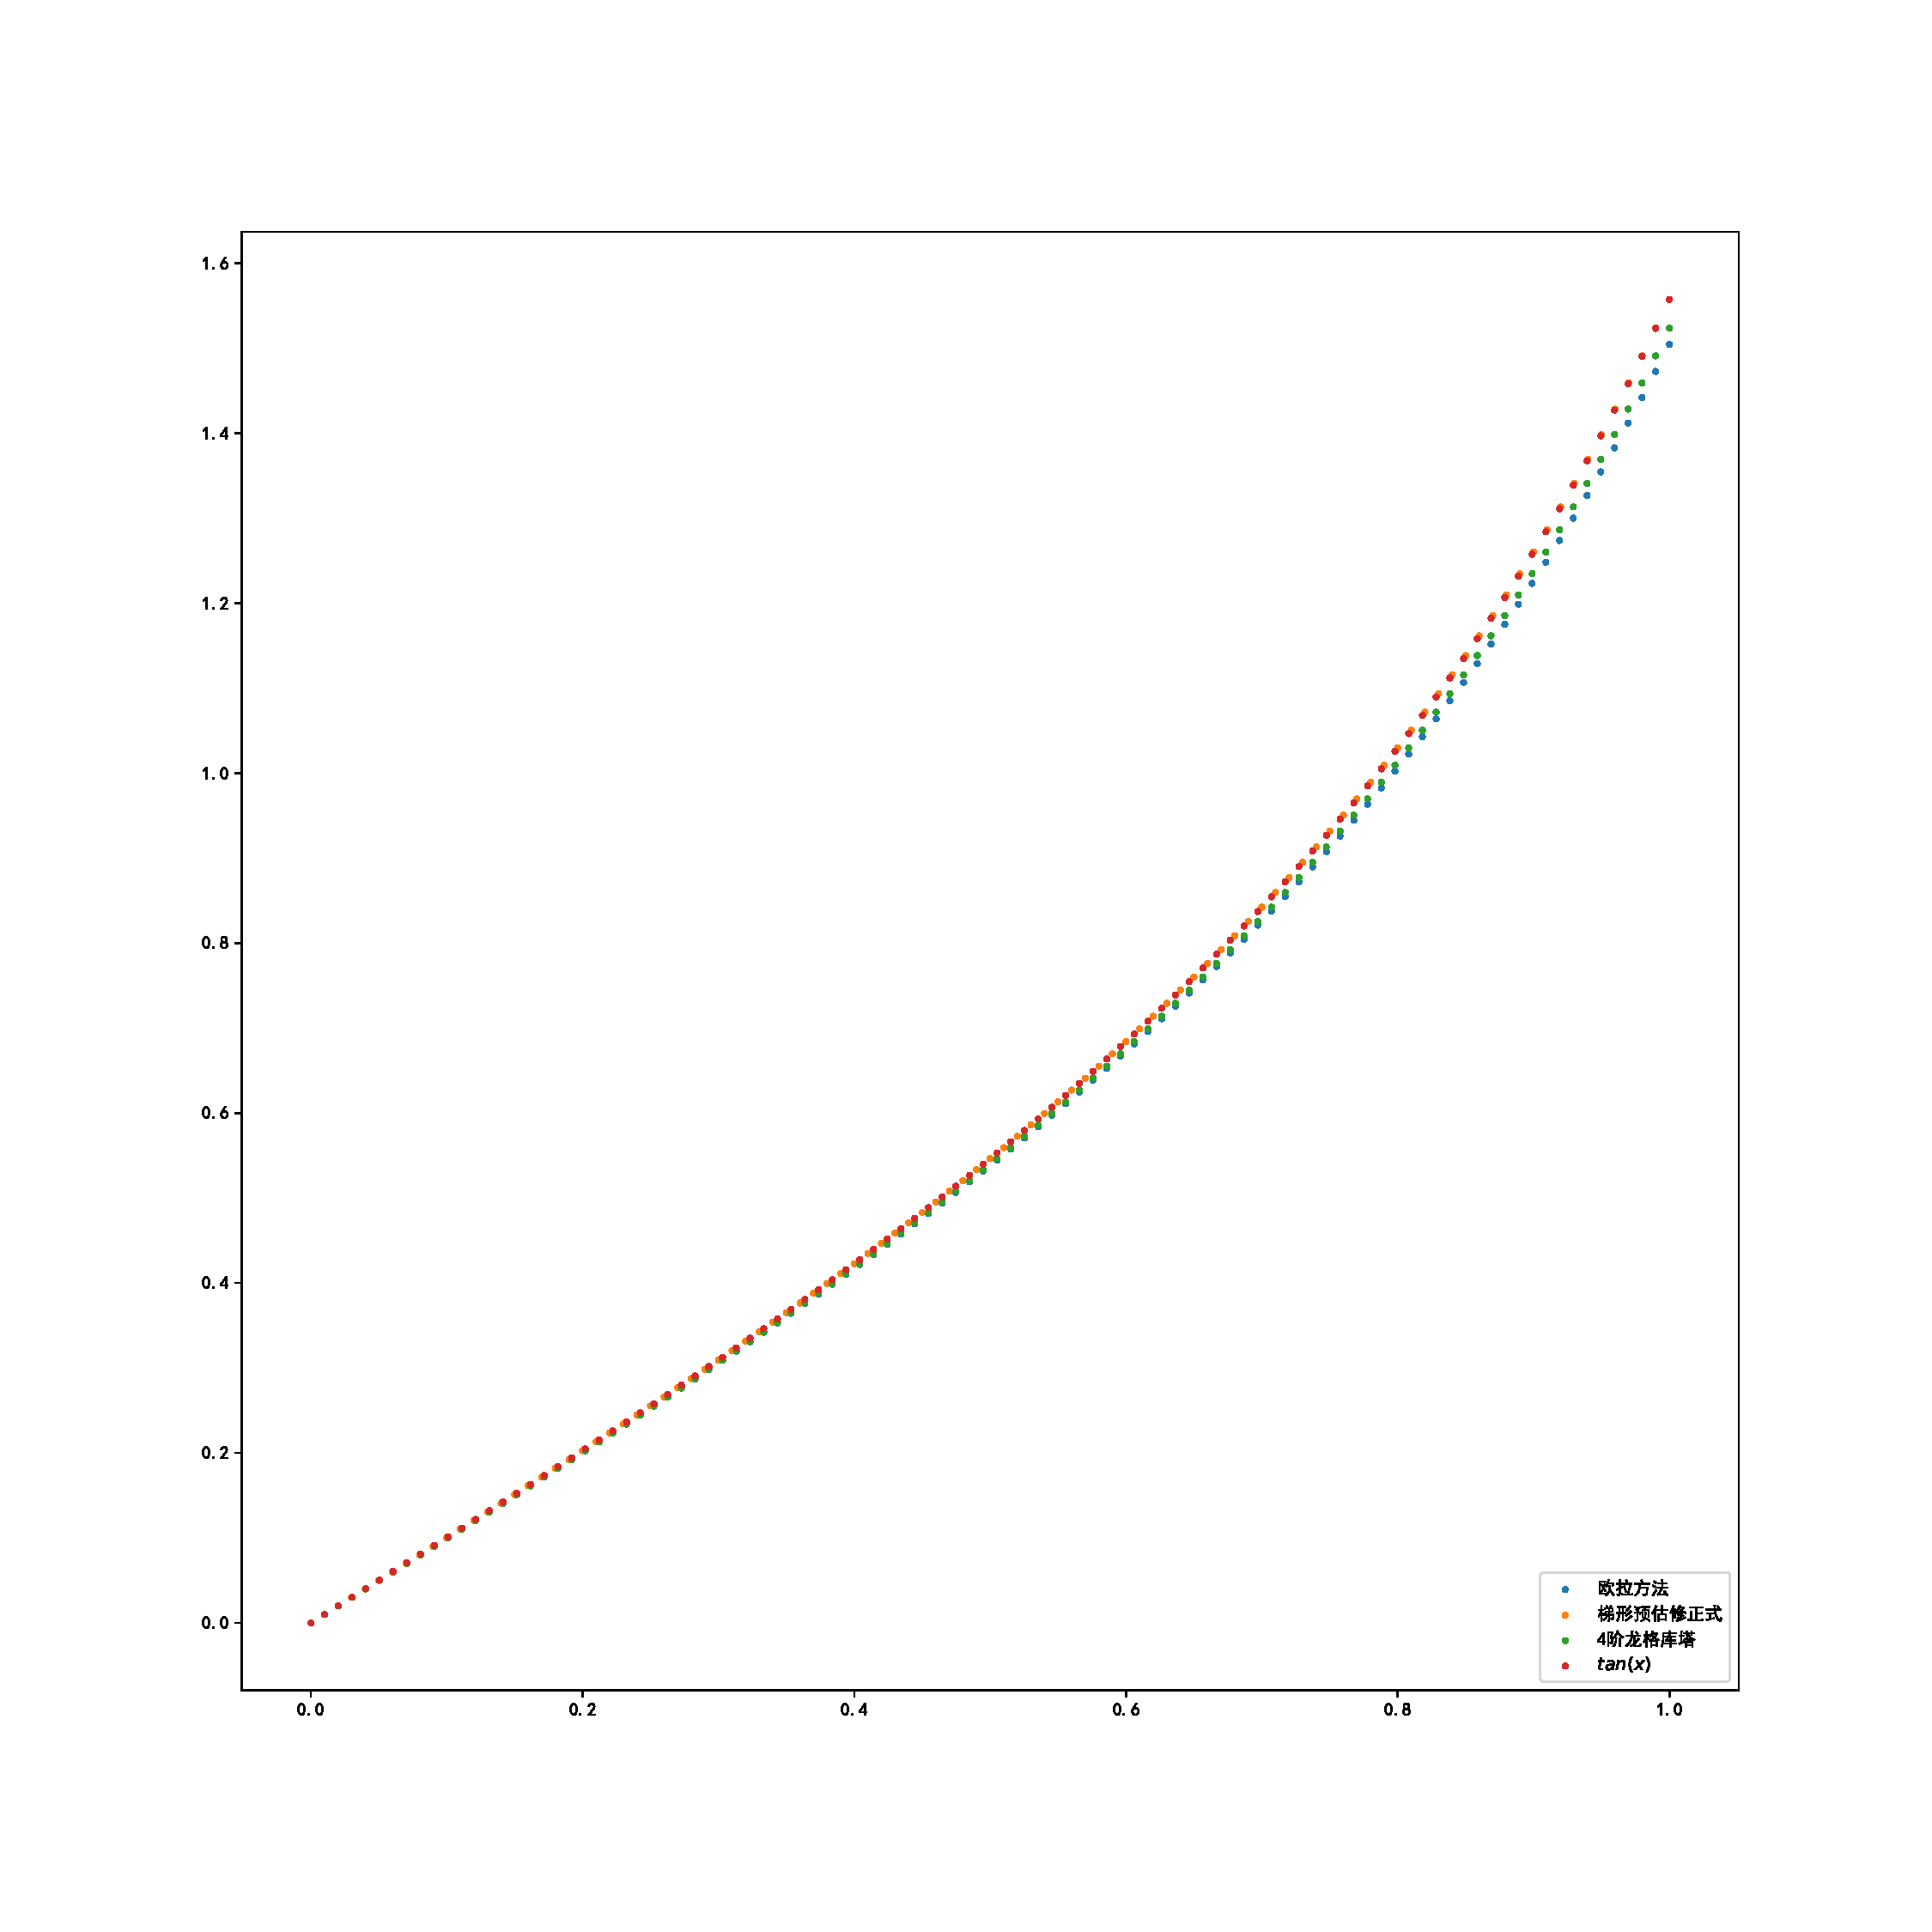
\includegraphics[width=\linewidth]{6-4.pdf}
\end{figure}


\paragraph{代码}

\begin{minted}{python}

def f(y):
    return 1+y**2


def euler(t, y0, a, b):
    t = np.linspace(a, b, M)
    y = np.zeros(M)
    y[0] = y0
    for k in range(M - 1):
        y[k + 1] = y[k] + h * f(y[k])
        
def rk4(f, a, b, ya, M):
    h = (b - a) / M
    T = np.linspace(a, b, M)
    Y = np.zeros(M)
    Y[0] = ya
    for j in range(M - 1):
        k1 = h * f(T[j], Y[j])
        k2 = h * f(T[j] + h / 2, Y[j] + k1 / 2)
        k3 = h * f(T[j] + h / 2, Y[j] + k2 / 2)
        k4 = h * f(T[j] + h, Y[j] + k3)
        Y[j + 1] = Y[j] + (k1 + 2 * k2 + 2 * k3 + k4) / 6
    return T, Y

def improved_euler(f,a=0,b=1,ya=1,h=0.1,verbose=True):
    res = []
    xi = a 
    yi = ya
    
    
    while xi <= b: # 在求解区间范围
        yp = yi + h*f(xi, yi)
        y = yi + h/2 * (f(xi, yi) + f(xi, yp))
        if verbose:
            xxx.append(xi)
            yyy.append(yi)
            #print('xi:{:.4f}, yi:{:.6f}'.format(xi,yi))
        res.append(y)
        xi, yi = xi+h, y
    
    return res
    
plt.figure(figsize=(15, 15))
#plt.subplot(1, 2, 1)
#T, Y = rk4(f, 0, 1.0, 0, 1000)
x=np.linspace(0,1,100)
plt.scatter(t, y, label='欧拉方法',s=6)
plt.scatter(xxx, yyy, label='梯形预估修正式',s=6)
plt.scatter(T, Y, label='4阶龙格库塔',s=6)
plt.scatter(x, np.tan(x), label='$tan(x)$',s=6)
plt.legend(loc='lower right')
plt.savefig('6-4.pdf')

\end{minted}

\subsection{题目2}
用龙格库塔4阶方法求解描述振荡器的经典van der Pol微分方程
$$\left\{
\begin{aligned}
\frac{d^2y}{dt^2}-\mu(1-y^2)\frac{dy}{dt}+y=0,\\
y(0)=1,y'(0)=0
\end{aligned}
\right.$$
分别取$\mu=0.01,0.1,1$作图比较计算结果

\paragraph{解答}
通过python实现四阶龙格库塔方法并作图得:

\begin{figure}[H]
	\centering
	\caption{四阶龙格库塔方法}
	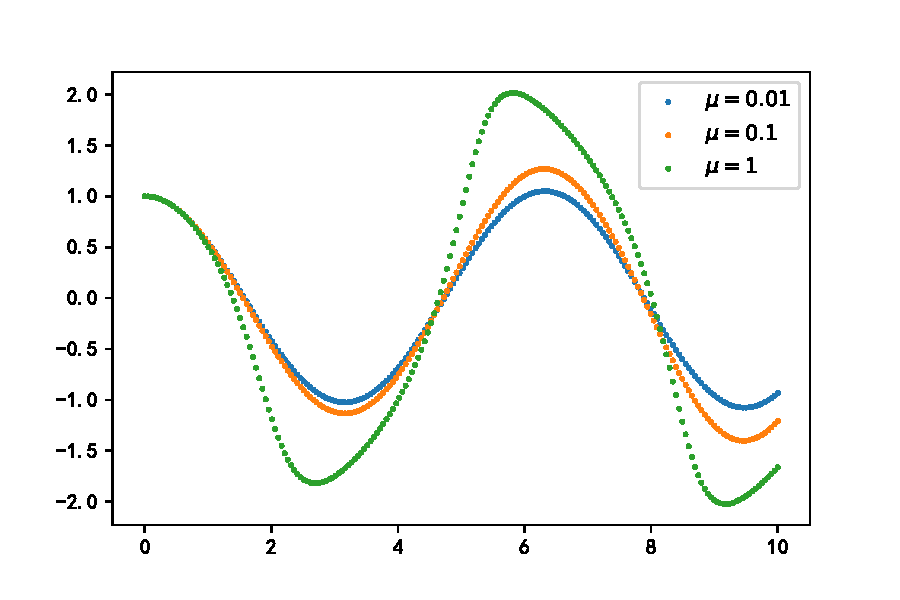
\includegraphics[width=\linewidth]{6-5.pdf}
\end{figure}

\paragraph{代码}


\begin{minted}{python}
def ff1(w1, w2):
    return 0.01*(1-w1*w1)*w2-w1

def ff2(w1, w2):
    return 0.1*(1-w1*w1)*w2-w1

def ff3(w1, w2):
    return 1*(1-w1*w1)*w2-w1


def rk42(f, w1, w2, h, a, b):  # f:二阶导函数 w1: 函数值 w2:一阶导数值 a,b:范围
    M = int((b-a)/h)
    T1 = np.linspace(a, b, int(M))
    Y1 = np.zeros(M)
    Y2 = np.zeros(M)
    Y1[0] = w1
    Y2[0] = w2
    for j in range(M - 1):
        k11 = h * Y2[j]
        k12 = h * f(Y1[j], Y2[j])
        k21 = h * (Y2[j] + 0.5 * k12)
        k22 = h * f(Y1[j]+0.5*k11, Y2[j]+0.5*k12)
        k31 = h * (Y2[j]+0.5*k22)
        k32 = h * f(Y1[j]+0.5*k21, Y2[j]+0.5*k22)
        k41 = h * (Y2[j]+0.5*k32)
        k42 = h * f(Y1[j]+0.5*k31, Y2[j]+0.5*k32)
        #print(Y1[j])
        Y1[j+1] = Y1[j]+(k11+2*k21+2*k31+k41)/6
        Y2[j + 1] = Y2[j] + (k12 + 2 * k22 + 2 * k32 + k42) / 6

    return Y1, Y2

ydot1,mmm=rk42(ff1,1,0,0.05,0,10)
ydot2,mmm=rk42(ff2,1,0,0.05,0,10)
ydot3,mmm=rk42(ff3,1,0,0.05,0,10)
plt.rcParams['figure.dpi'] = 200
xdot= np.linspace(0, 10, 200)
plt.scatter(xdot, ydot1,label='$\mu=0.01$',s=2)
plt.scatter(xdot, ydot2,label='$\mu=0.1$',s=2)
plt.scatter(xdot, ydot3,label='$\mu=1$',s=2)
plt.legend()
plt.savefig('6-5.pdf',dpi=200)

\end{minted}


